\section{Introduction}
The recent commercial availablity of relatively cheap mobile robots such 
as Baxter and the UBR 1 creates a very real possiblity for widespread 
appliation of robotics to mobile manipulation tasks.
There are huge economic gains to be had from the deployment of robotics 
in settings that range from homes to factories.
Our goal is to endow robots with the ability to execute complex, goal-directed, 
tasks in these unstructured settings.

In particular, deformable object manipulation presents an interesting challenge.
These problems are characterized by state and action spaces that are high-dimensional 
and continuous and direct solutions require reasoning about dynamics of complex object 
through contact.
Determing a correct underlying representation of these objects is itself a difficult problem,
and current approaches require complicated task specific implementations.

Learning from demonstrations provides a way to sidestep these issues:
rather than starting from scratch in each scenario, we generalize from 
an expert demonstration.
If it can be done robustly, adapting an example trajecotry to a new scene 
gives an easy way for lay people to provide custom solutions a wide variety of tasks
well beyond the state-of-the-art.

A recent approach makes use of \emph{trajectory transfer} through the use of non-rigid registration to solve this problem.
Trajectory tranfers fits a function $f:\mathbb{R}^3 \rightarrow \mathbb{R}^3$ that warps a demonstration scene to a novel setting.
The demonstrated trajectory is warped with this function and the result is executed. 
This has been shown to be effective for many complex task, including knot-tying and suturing \cite{Schulmanetal_ISRR2013, Schulmanetal_IROS2013}.

This approach has its limits.
A single demonstration cannot be expected to cover all possible scenarios.
The natural solution to this is to use a library of demonstrations.
In addition to increasing the number of state we can generalize to trajectory libraries
enable the generalization beyond the demonstrations to complex tasks by sequencing 
several trajecotry generalizations.

However, realizing these benefits requires a robost technique to select a good trajectory to
transfer.
This is not an easy task.
Certain trajectories will generalize better than others and particular sequences of 
demonstrations may perform tasks more efficiently than others.
Furthermore, the existence of poor or brittle demonstrations can very negatively 
effect performance.

\begin{figure}[t]
  \centering
    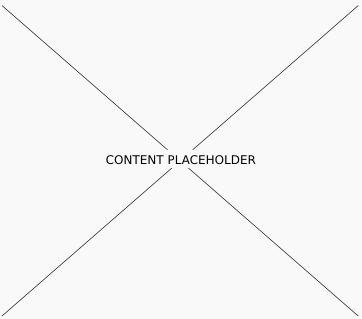
\includegraphics[width=0.9\linewidth]{figures/placeholder.png}
  \caption{Cute picture of robot tying knot}
  \label{fig:frontfig}
\end{figure}

In this paper, we present a solution to the demonstration selection problem that can 
account for the generalizability of demonstrations and the sequential nature of our 
applications.
Given a set of demonstrations and a method for generalizing them, we construct a 
discrete-action abstract MDP.
Each action in this MDP is associated with a demonstration and our transition 
function is defined as applying trajectory transfer to generalize that demonstration.

This construction allows us to learn a Q function from example sequences of 
state and demonstration pairs.
Our Q-function learning is done through a novel Learning from Demonstrations
technique that accounts for both the optimality of the expert trajecotries and the
sequenatial nature of the task.
We call this approach Max-Margin Q Learning, {\sc mmql}.

Our approach relies only on features which are completely task 
agnostic and can be applied to any problem where trajectory transfer applies. 
We investigate the utility of this approach in a challenging knot-tieing scenario 
and show that the greedy application of our learned policy strongly outperforms the 
\citet{Schulmanetal_ISRR2013}'s nearest-neighbor method on a challenging distribution of 
problems. 
We leverage the fact that we learn a Q function representation of our policy (as 
opposed to a direct mapping from features to actions) to use a beam search to get 
near perfect performance in this task.
Finally, we present a method for bootstraping, though a process we call Leave-One-Out-Labelling, that enables us to do Max Margin Q-Learning with no additional human supervision beyond the initial demonstrations.

The rest of this paper is organized as follows: \dhm{we will fill this in later}


